\sectionframe{3. Conditional Firm-Size Premiums}

\begin{frame}{Start with the Simplest Specification}
  \[
  \ln w_{ist}=\alpha+\sum_{g\ne g_0}\beta_g D_{ig}+\varepsilon_{ist}.
  \]
  \begin{enumerate}
    \item Start with firm-size indicators alone.
    \item Add sector-year fixed effects.
    \item Add sex, age, age squared, and education.
    \item Add formality as a level control.
  \end{enumerate}
  \vspace{0.2cm}
  \idea{This sequence still imposes the same size coefficients on formal and informal workers.}
  %\source{Paper Table~\paperref{tab:firm-size-wage-premium-regressions}. $g_0$ denotes solo work. Column (4) estimates Equation~(\paperref{eq:common-premium}). All columns use the same 5,268,514 observations.}
\end{frame}

\begin{frame}{Adding Controls Reduces the 101+/Solo Premium}
  \centering\begingroup\fontsize{8.5}{10}\selectfont
  \setlength{\tabcolsep}{4pt}
  \begin{adjustbox}{max width=\textwidth,max totalheight=0.68\textheight}
    \begin{tabular}{lcccc}
\toprule
    & \multicolumn{4}{c}{Dependent variable: log real hourly labor income} \\
    \cmidrule(lr){2-5}
    & (1) & (2) & (3) & (4) \\
    \midrule
Firm size: 2-3 & 0.184*** \sereg{0.034} & 0.242*** \sereg{0.031} & 0.209*** \sereg{0.027} & 0.188*** \sereg{0.029} \\
Firm size: 4-5 & 0.363*** \sereg{0.034} & 0.408*** \sereg{0.030} & 0.361*** \sereg{0.029} & 0.307*** \sereg{0.038} \\
Firm size: 6-10 & 0.499*** \sereg{0.029} & 0.500*** \sereg{0.033} & 0.422*** \sereg{0.037} & 0.316*** \sereg{0.050} \\
Firm size: 11-19 & 0.625*** \sereg{0.034} & 0.575*** \sereg{0.040} & 0.457*** \sereg{0.042} & 0.302*** \sereg{0.050} \\
Firm size: 20-30 & 0.687*** \sereg{0.046} & 0.603*** \sereg{0.045} & 0.462*** \sereg{0.046} & 0.271*** \sereg{0.051} \\
Firm size: 31-50 & 0.759*** \sereg{0.056} & 0.650*** \sereg{0.049} & 0.487*** \sereg{0.047} & 0.271*** \sereg{0.048} \\
Firm size: 51-100 & 0.818*** \sereg{0.063} & 0.698*** \sereg{0.051} & 0.518*** \sereg{0.048} & 0.289*** \sereg{0.047} \\
Firm size: 101+ & 1.017*** \sereg{0.102} & 0.817*** \sereg{0.067} & 0.598*** \sereg{0.061} & 0.359*** \sereg{0.059} \\
\midrule
    Gender, age, and education controls & No & No & Yes & Yes \\
Formality control & No & No & No & Yes \\
Sector-year fixed effects & No & Yes & Yes & Yes \\
Observations & 5,268,514 & 5,268,514 & 5,268,514 & 5,268,514 \\
$R^2$ & 0.213 & 0.271 & 0.376 & 0.386\\
\bottomrule\end{tabular}

  \end{adjustbox}\endgroup
  \par\vspace{0.15cm}
  {\small The 101+/solo coefficient falls from 1.017 to 0.359 log points. The latter corresponds to a 43.2\% premium.}
  \source{Paper Table~\paperref{tab:firm-size-wage-premium-regressions}. Reference is solo work. Sector-clustered SEs in parentheses. * $p<0.10$, ** $p<0.05$, *** $p<0.01$.}
\end{frame}

\begin{frame}{Then Add Geography and Occupational Position}
  \centering\begingroup\fontsize{8.5}{10}\selectfont
  \setlength{\tabcolsep}{4pt}
  \begin{adjustbox}{max width=\textwidth,max totalheight=0.68\textheight}
    \begin{tabular}{lcccc}
\toprule
    & \multicolumn{4}{c}{Dependent variable: log real hourly labor income} \\
    \cmidrule(lr){2-5}
    & (1) & (2) & (3) & (4) \\
    \midrule
Firm size: 2-3 & 0.188*** \sereg{0.011} & 0.168*** \sereg{0.011} & 0.167*** \sereg{0.011} & 0.102*** \sereg{0.013} \\
Firm size: 4-5 & 0.307*** \sereg{0.014} & 0.277*** \sereg{0.014} & 0.273*** \sereg{0.014} & 0.225*** \sereg{0.015} \\
Firm size: 6-10 & 0.316*** \sereg{0.018} & 0.282*** \sereg{0.017} & 0.278*** \sereg{0.017} & 0.265*** \sereg{0.016} \\
Firm size: 11-19 & 0.302*** \sereg{0.018} & 0.272*** \sereg{0.017} & 0.267*** \sereg{0.017} & 0.272*** \sereg{0.015} \\
Firm size: 20-30 & 0.271*** \sereg{0.019} & 0.241*** \sereg{0.017} & 0.237*** \sereg{0.017} & 0.258*** \sereg{0.015} \\
Firm size: 31-50 & 0.271*** \sereg{0.018} & 0.245*** \sereg{0.017} & 0.240*** \sereg{0.017} & 0.263*** \sereg{0.015} \\
Firm size: 51-100 & 0.289*** \sereg{0.018} & 0.262*** \sereg{0.017} & 0.257*** \sereg{0.017} & 0.282*** \sereg{0.015} \\
Firm size: 101+ & 0.359*** \sereg{0.023} & 0.338*** \sereg{0.024} & 0.325*** \sereg{0.024} & 0.338*** \sereg{0.022} \\
\midrule
    Worker and formality controls & Yes & Yes & Yes & Yes \\
Occupational-position controls & No & No & No & Yes \\
Fixed effects & $s\times t$ & $s\times t$, $d\times t$ & $s\times d\times t$ & $s\times d\times t$ \\
Observations & 5,268,514 & 5,268,514 & 5,268,375 & 5,268,375 \\
$R^2$ & 0.386 & 0.404 & 0.414 & 0.429\\
\bottomrule\end{tabular}

  \end{adjustbox}\endgroup
  \par\vspace{0.15cm}
  {\small The final 101+/solo coefficient is 0.338, or 40.2\%. But should one size premium describe both formal and informal employment?}
  %\source{Paper Table~\paperref{tab:firm-size-local-geography-robustness}. Column (4) estimates Equation~(\paperref{eq:common-premium-geography}). SEs cluster by sector-department. Columns (3)--(4) exclude 139 singleton observations.}
\end{frame}

\begin{frame}{The Preferred Specification}
  \small
  \begin{align*}
  \ln w_{iosdt}={}&\alpha+\phi F_i+
    \sum_{g\ne g_0}(\beta_g+\theta_g F_i)D_{ig}\\
    &+X_i'\gamma+\rho_o+\lambda_{s\times d\times t}+\varepsilon_{iosdt}.
  \end{align*}
  \begin{itemize}
    \item $F_i$ indicates pension contribution. $D_{ig}$ indicates firm-size category.
    \item $X_i$ includes sex, age, age squared, and education.
    \item $\rho_o$ controls for occupational position, including own-account work.
    \item $\lambda_{s\times d\times t}$ compares workers within the same sector, department, and year.
    \item Solo work is the reference within each formality group: $\beta_{g_0}=\theta_{g_0}=0$.
  \end{itemize}
  %\source{Paper Equation~(\paperref{eq:main}) and Table~\paperref{tab:firm-size-local-geography-formality-robustness}, column (4). 5,268,375 observations. Baseline inference uses 559 sector-department clusters.}
\end{frame}

\begin{frame}{What the Coefficients Compare}
  \begin{center}
  \small
  \begin{tabular}{lll}
  \toprule
  Log-income comparison & Contrast & Coefficients \\
  \midrule
  Informal, size $g$ to $h$ & $\Delta^I_{g\to h}$ & $\beta_h-\beta_g$ \\
  Formal, size $g$ to $h$ & $\Delta^F_{g\to h}$ & $(\beta_h+\theta_h)-(\beta_g+\theta_g)$ \\
  Informal to formal, size $g$ & $\Delta^{I\to F}_g$ & $\phi+\theta_g$ \\
  \bottomrule
  \end{tabular}
  \end{center}
  \vspace{0.25cm}
  \begin{itemize}
    \item For each estimated contrast $\widehat\Delta$, report $100[\exp(\widehat\Delta)-1]$.
    \item These are ratios of exponentiated conditional mean log incomes, not necessarily ratios of arithmetic means.
  \end{itemize}
  %\source{Paper Equation~(\paperref{eq:preferred-contrasts}). Changing the reference category leaves fitted values and pairwise comparisons unchanged.}
\end{frame}

\begin{frame}{Preferred Regression Output}
  \centering\small
  \begin{tabular}{lcc}
  \toprule
  Firm size & Informal: $\widehat\beta_g$ & Formal: $\widehat\beta_g+\widehat\theta_g$ \\
  \midrule
  2--3 & 0.113*** \sereg{0.013} & -0.072** \sereg{0.029} \\
  4--5 & 0.255*** \sereg{0.016} & -0.022 \sereg{0.033} \\
  6--10 & 0.324*** \sereg{0.017} & 0.013 \sereg{0.034} \\
  11--19 & 0.354*** \sereg{0.018} & 0.039 \sereg{0.032} \\
  20--30 & 0.362*** \sereg{0.017} & 0.039 \sereg{0.031} \\
  31--50 & 0.363*** \sereg{0.020} & 0.059* \sereg{0.031} \\
  51--100 & 0.372*** \sereg{0.020} & 0.085*** \sereg{0.031} \\
  101+ & 0.316*** \sereg{0.019} & 0.153*** \sereg{0.037} \\
  \bottomrule
  \end{tabular}
  \par\vspace{0.25cm}
  {\small Reference: solo workers of the same formality status.}
  \regnote{Log-point contrasts, not percent premiums. Standard errors in parentheses are clustered by sector-department. * $p<0.10$, ** $p<0.05$, *** $p<0.01$.}
\end{frame}

\begin{frame}{Adjusted Premiums by Formality}
  \centering
  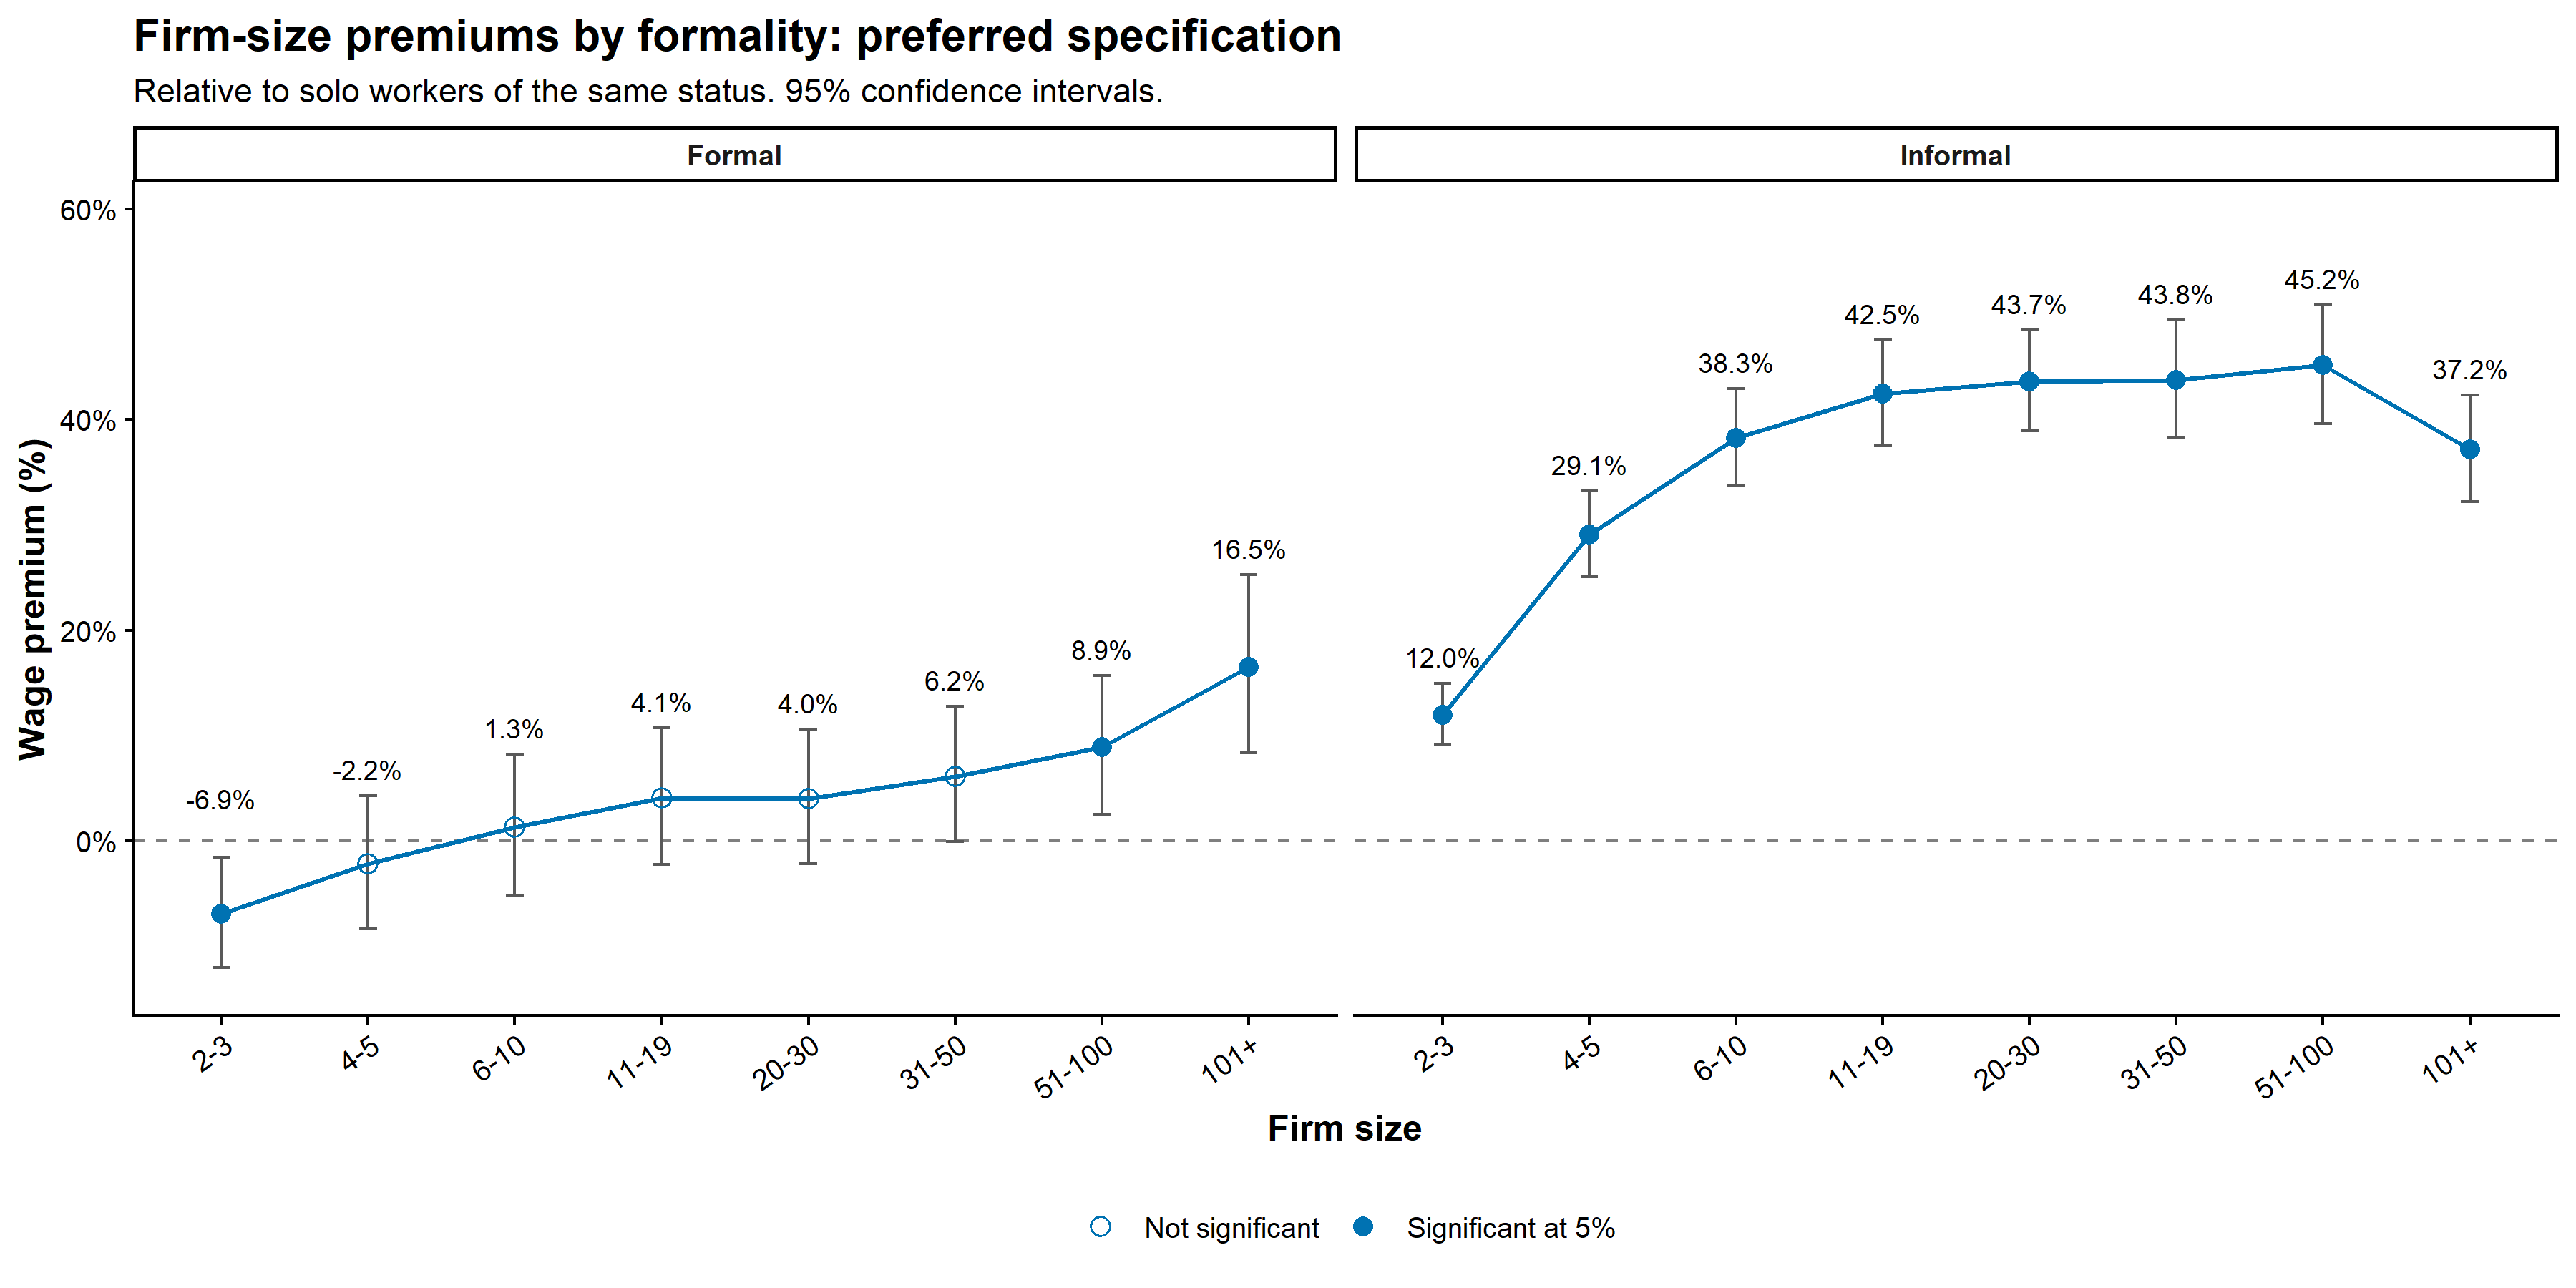
\includegraphics[width=0.98\textwidth,height=0.80\textheight,keepaspectratio]{preferred_formality_premiums_en.png}
  \source{Paper Figure~\paperref{fig:preferred-formality-premium}, Equation~(\paperref{eq:main}). Reference is solo work within formality. Bars use sector-department clustering. Alternative clustering is reported in the appendix.}
\end{frame}

\begin{frame}{The Comparison Depends on the Starting Size}
  \centering
  \begin{tabular}{lrr}
  \toprule
  Conditional wage comparison & Formal & Informal \\
  \midrule
  101+ relative to solo & 16.5\% & 37.1\% \\
  101+ relative to 11--19 & 12.0\% & -3.7\% \\
  \bottomrule
  \end{tabular}
  \par\vspace{0.4cm}
  \begin{itemize}
    \item The formal 101+ advantage over categories from 2--3 through 51--100 remains significant with alternative clustering.
    \item Informal premiums rise sharply across the smallest sizes, then flatten and fall at 101+.
    \item A larger informal 101+/solo premium does not imply gains at every step toward larger firms.
  \end{itemize}
  \source{Paper Tables~\paperref{tab:firm-size-local-geography-formality-robustness}--\paperref{tab:firm-size-local-geography-formality-robustness-11-19-reference}. The informal 101+/11--19 contrast is not significant at 5\% with sector or two-way clustering.}
\end{frame}

\begin{frame}{Formal Workers Earn More at Each Firm Size}
  \centering\small
  \begin{tabular}{lrrrrrrrrr}
  \toprule
  Size & Solo & 2--3 & 4--5 & 6--10 & 11--19 & 20--30 & 31--50 & 51--100 & 101+ \\
  \midrule
  Gap (\%) & 59.3 & 32.4 & 20.8 & 16.8 & 16.4 & 15.4 & 17.7 & 19.6 & 35.4 \\
  \bottomrule
  \end{tabular}
  \par\vspace{0.4cm}
  \begin{itemize}
    \item These contrasts hold firm size fixed, unlike the preceding figure.
    \item All nine gaps remain positive and significant under every clustering procedure examined.
    \item The size premium is not just a comparison between formal and informal jobs.
  \end{itemize}
  \source{Paper Table~\paperref{tab:preferred-formality-gap}. Formal relative to informal workers, conditional on preferred controls. These are associations, not effects of formalization.}
\end{frame}

\sectionframe{4. Dynamics and Elasticities}

\begin{frame}{Has the Conditional Premium Changed?}
  \small
  \begin{align*}
    \ln w_{iosdt}={}&\sum_{\tau\in\mathcal T}\mathbf{1}\{t=\tau\}
    \left[\phi_\tau F_i+\sum_{g\ne g_0}(\beta_{g\tau}+\theta_{g\tau}F_i)D_{ig}
    +X_i'\gamma_\tau+\rho_{o\tau}\right]\\
    &+\lambda_{s\times d\times t}+\varepsilon_{iosdt}.
  \end{align*}
  \begin{itemize}
    \item All size, formality, worker-control, and occupational-position coefficients vary by year.
    \item Annual profiles come from separate yearly regressions.
    \item Test 2008--2025 changes jointly, retaining cross-year covariance within clusters.
  \end{itemize}
  \vspace{0.2cm}
  \idea{All change tests are two-sided. Widening and narrowing are both possible.}
  \source{Paper Equation~(\paperref{eq:preferred-dynamics}). $\mathcal T$ is the set of sample years. Endpoint tests are pointwise, without multiple-testing adjustment.}
\end{frame}

\begin{frame}{Adjusted Profiles in 2008 and 2025}
  \centering
  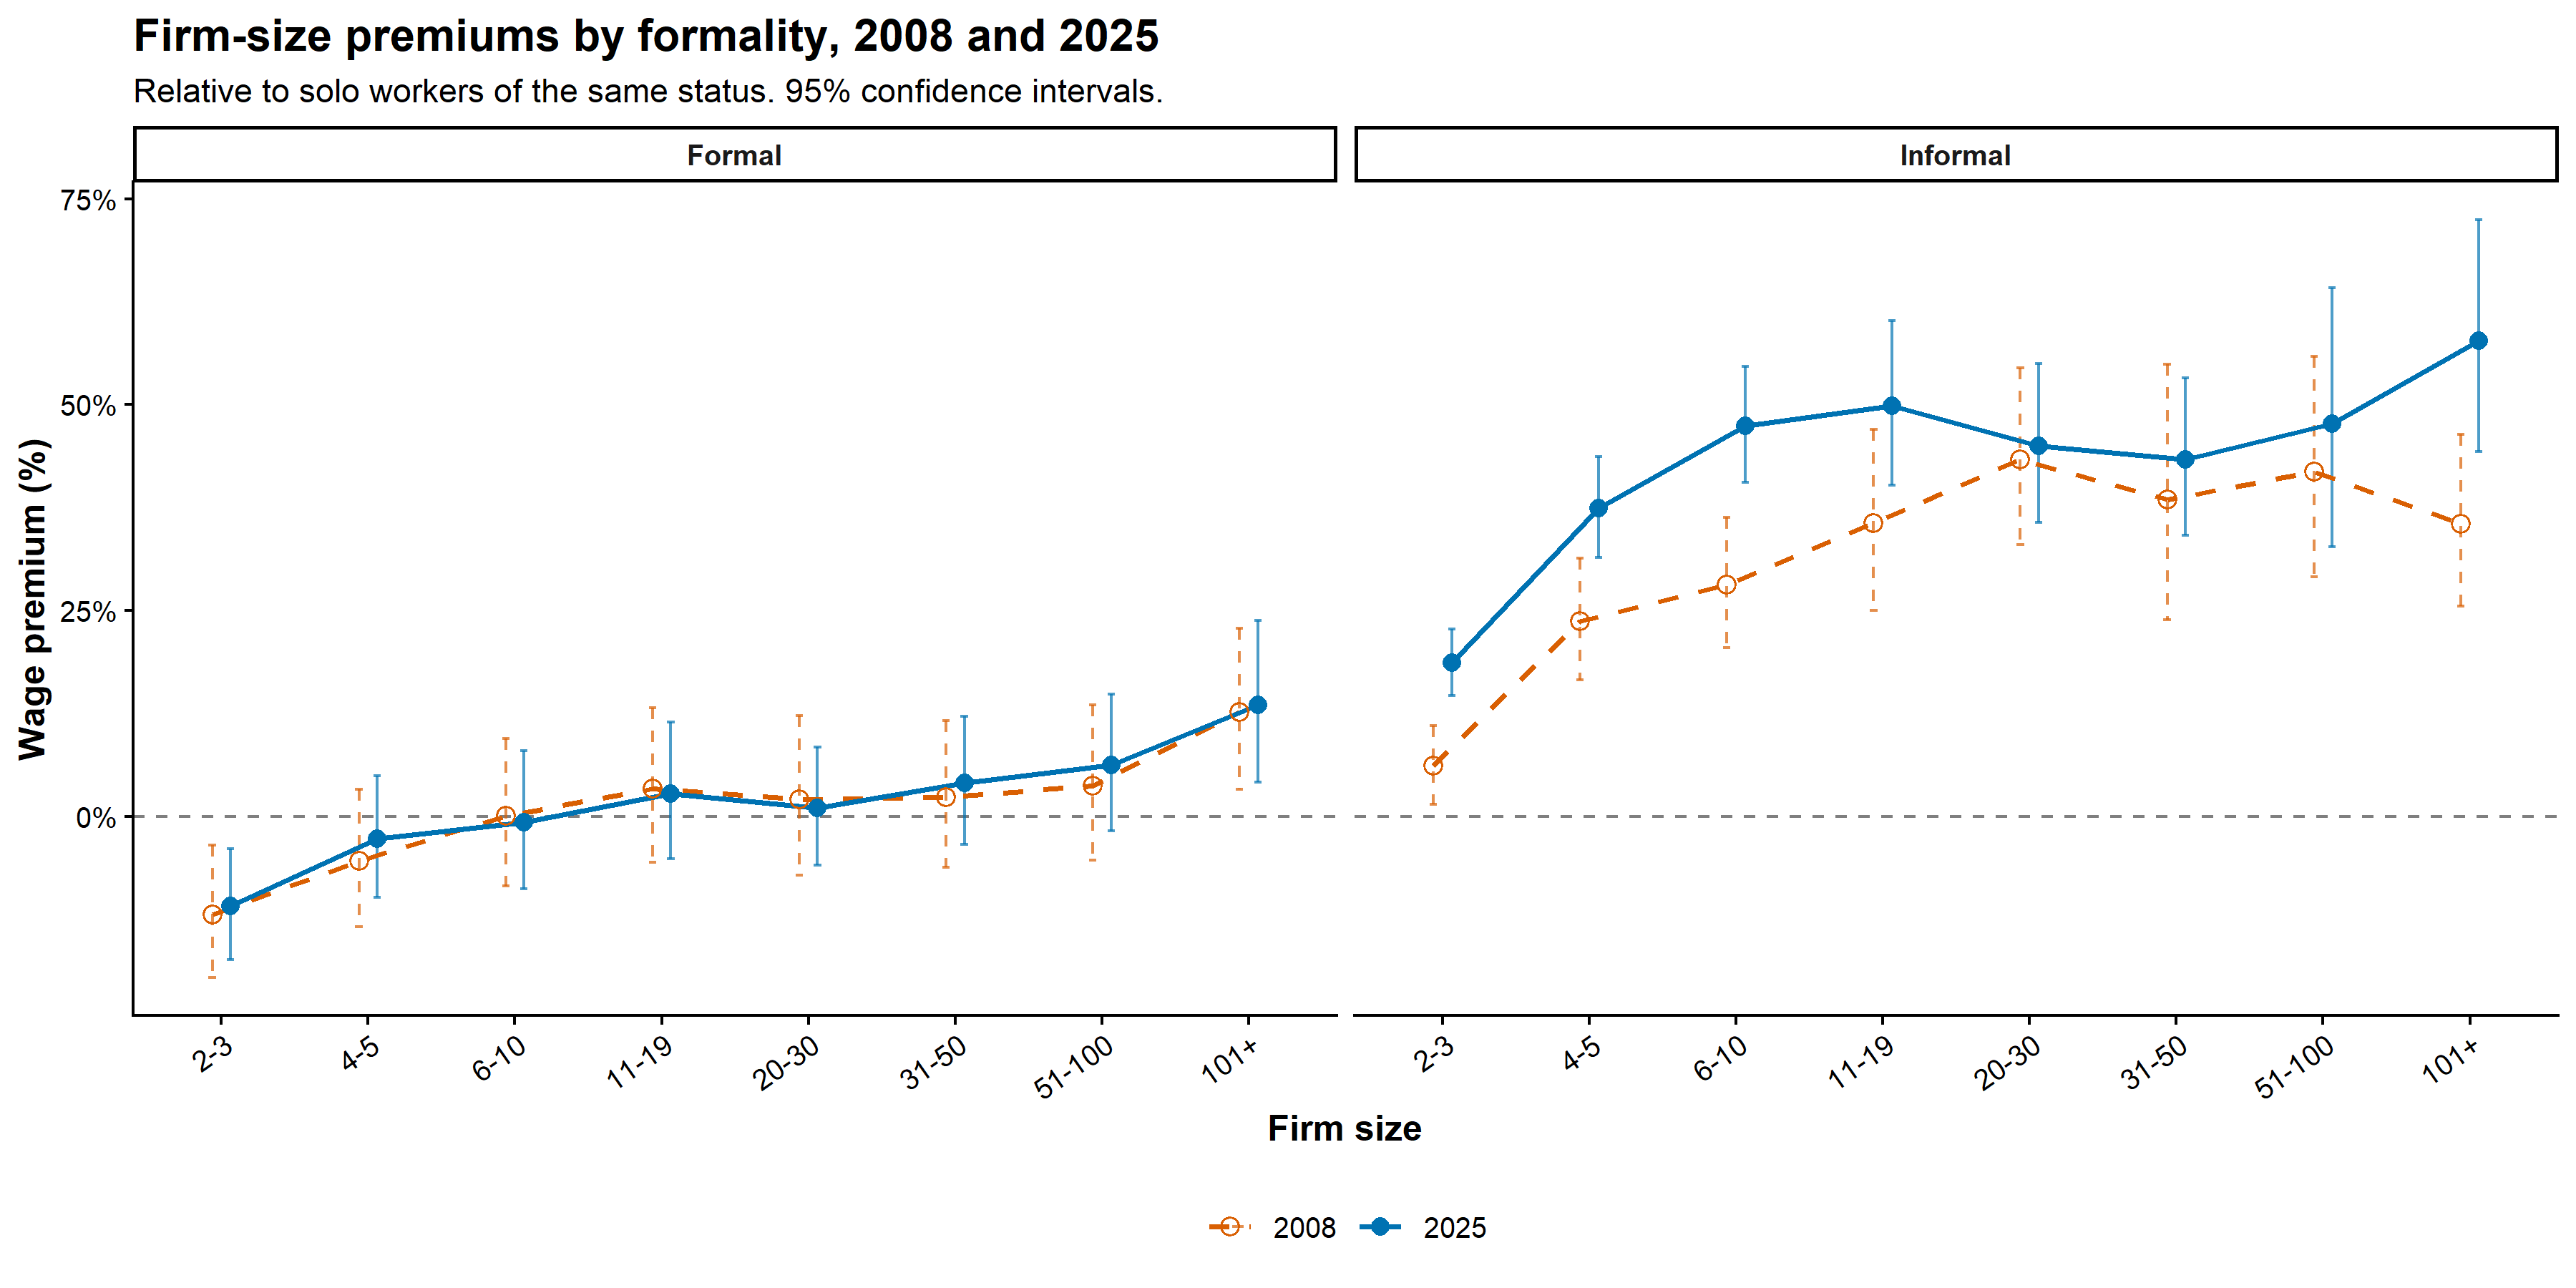
\includegraphics[width=0.98\textwidth,height=0.80\textheight,keepaspectratio]{preferred_formality_endpoints_en.png}
  \source{Paper Figure~\paperref{fig:preferred-formality-endpoints}, Equation~(\paperref{eq:preferred-dynamics}). Reference is solo work within each formality-year group. Intervals use sector-department clustering.}
\end{frame}

\begin{frame}{Endpoint Changes Differ by Formality}
  \small\centering
  \begin{tabular}{lrrrr}
  \toprule
  101+/solo premium & 2008 & 2025 & Change (pp) & \shortstack{$p$-value\\Sector-department} \\
  \midrule
  Formal & 12.6\% & 13.5\% & 0.9 & 0.861 \\
  Informal & 35.6\% & 57.7\% & 22.2 & 0.011 \\
  \bottomrule
  \end{tabular}
  \par\vspace{0.35cm}
  \begin{itemize}
    \item The formal premium ends the period close to its initial level. Its change is not significant.
    \item The informal estimate rises substantially, but the increase is not significant at 5\% with sector ($p=0.090$) or two-way clustering ($p=0.199$).
    \item The endpoint comparison is not a test of a steady linear trend.
  \end{itemize}
  \source{Paper Tables~\paperref{tab:preferred-endpoint-changes} and \paperref{tab:preferred-clustering-comparison}. Changes are computed before rounding. The table above reports baseline sector-department $p$-values.}
\end{frame}

\begin{frame}{The Annual Path Is Not a Steady Trend}
  \centering
  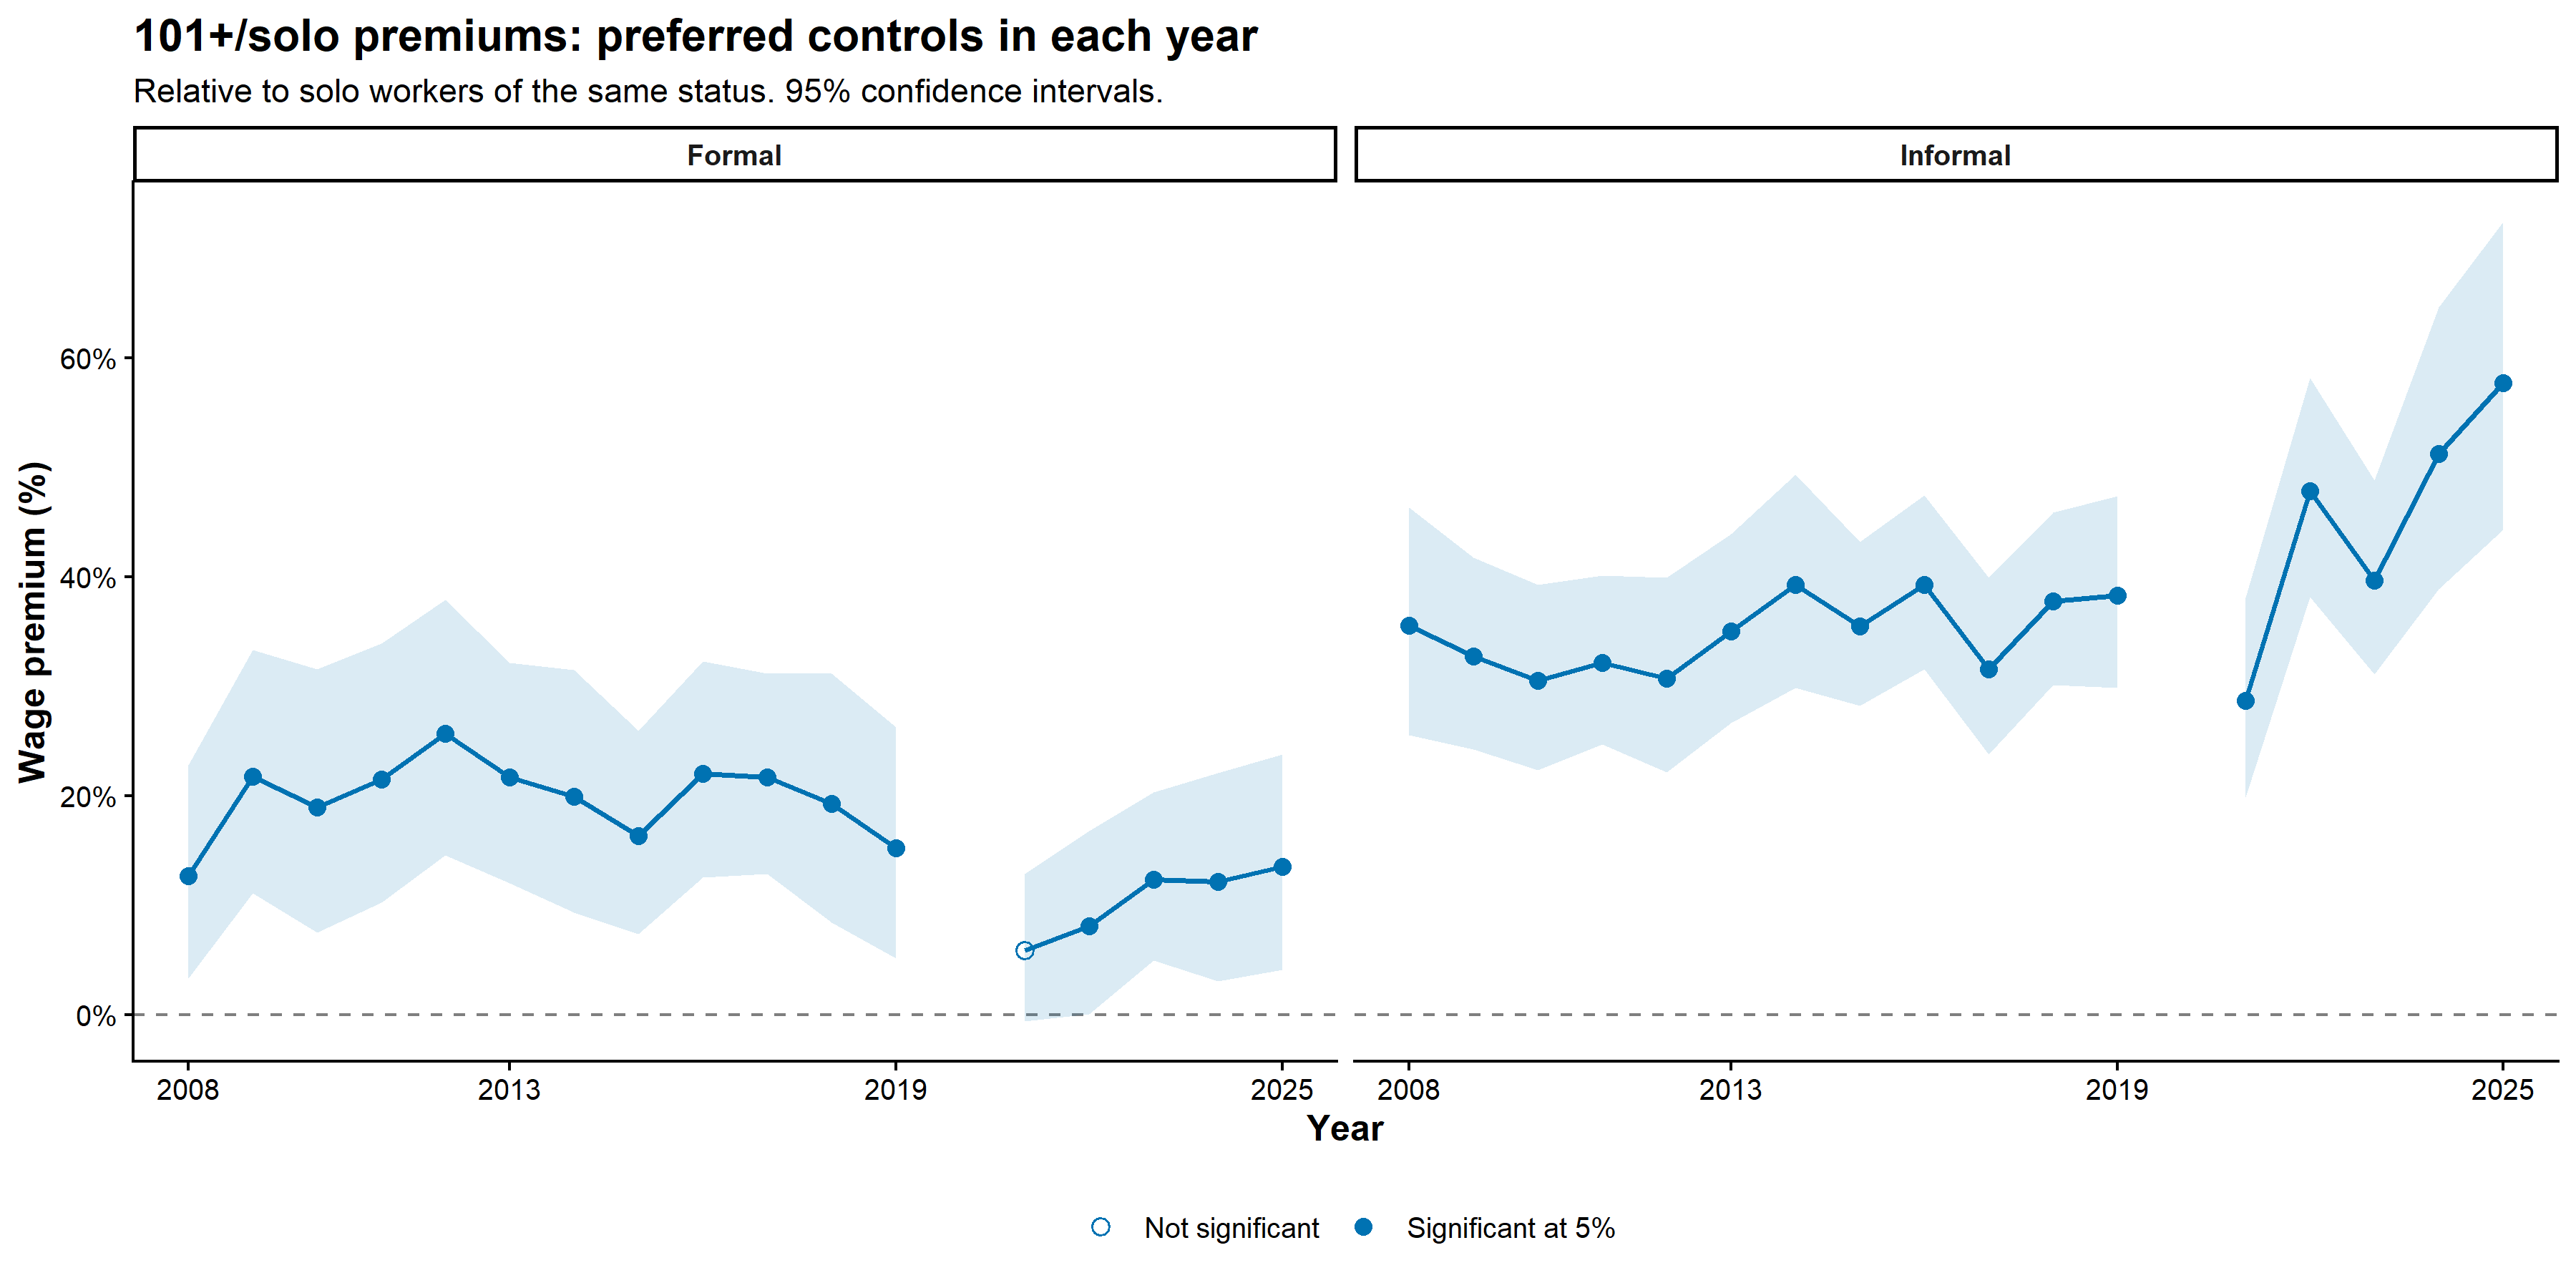
\includegraphics[width=0.98\textwidth,height=0.80\textheight,keepaspectratio]{preferred_large_firm_dynamics_en.png}
  \source{Paper Figure~\paperref{fig:preferred-large-firm-dynamics}, Equation~(\paperref{eq:preferred-dynamics}). Annual 101+/solo contrasts. Intervals use sector-department clustering. 2020 is excluded.}
\end{frame}

\begin{frame}{Contrast with Previous Evidence on Changes over Time}
  \begin{itemize}
    \item Bloom et al. (2018) document a declining large-firm premium in the United States.
    \item Reed and Tran (2019) report declines with national income and over time across developing economies.
    \item Colonnelli et al. (2018) find no common trajectory across Brazil, Germany, Sweden, and the United Kingdom.
    \item Colombia shows little net change in the formal endpoints. The informal estimate rises, but its significance at 5\% depends on the clustering procedure.
  \end{itemize}
  \source{The relevant comparison is the time path of size-related wage gaps, not the dispersion of firm-specific pay effects.}
\end{frame}

\begin{frame}{Why Estimate an Approximate Elasticity?}
  \small
  \[
  \begin{aligned}
  \ln w_{iosdt}={}&\alpha+\phi F_i+(\eta+\kappa F_i)\ln\widetilde{Size}_{iosdt}\\
       &+X_i'\gamma+\rho_o+\lambda_{s\times d\times t}+\varepsilon_{iosdt}.
  \end{aligned}
  \]
  \begin{itemize}
    \item A log-log slope provides a compact comparison with the literature.
    \item GEIH reports bins, not exact counts. Assign sizes of 1, 2.5, 4.5, 8, 15, 25, 40.5, 75.5, and 150.
    \item The informal slope is $\eta$. The formal slope is $\eta+\kappa$.
    \item Both slopes come from one regression with preferred controls, not separate samples.
  \end{itemize}
  \source{Paper Equation~(\paperref{eq:preferred-elasticity}). An assigned-size approximation. The categorical model does not impose a constant elasticity.}
\end{frame}

\begin{frame}{Benchmarking the Elasticities}
  \centering\small
  \setlength{\tabcolsep}{4pt}
  \begin{tabular}{p{0.29\textwidth}p{0.37\textwidth}cc}
\toprule
    Source & Specification & Elasticity & S.E. \\
    \midrule
Diegmann et al. (2026) & No worker controls & 0.062 & n.a. \\
Diegmann et al. (2026) & Observable worker controls & 0.036 & n.a. \\
\midrule
    Colombia (GEIH) & No controls & 0.205*** & (0.008) \\
Colombia (GEIH) & Common-slope model & 0.060*** & (0.004) \\
Colombia (GEIH) & Formal workers & 0.041*** & (0.005) \\
Colombia (GEIH) & Informal workers & 0.097*** & (0.004)\\
\bottomrule\end{tabular}

  \par\vspace{0.2cm}
  \begin{itemize}
    \item The informal slope exceeds the formal slope by $-\widehat\kappa=0.057$ ($p<0.001$ with two-way clustering).
    \item Different populations and controls limit the benchmark to a comparison of magnitudes.
  \end{itemize}
  \source{Paper Tables~\paperref{tab:preferred-elasticities} and \paperref{tab:preferred-clustering-comparison}. Displayed SEs use sector-department clustering. Literature means from Diegmann et al. (2026).}
\end{frame}

\sectionframe{5. Illustrative Income Scenarios}

\begin{frame}{What Would Income Be under Another Size or Formality?}
  \begin{itemize}
    \item Apply the pooled preferred coefficients to the 341,282 observations in the 2025 estimation sample.
    \item Change firm size, formality, or both.
    \item Keep characteristics, occupational position, sector, department, hours, and weights fixed.
    \item Workers already at the destination keep their baseline predictions.
  \end{itemize}
  \vspace{0.2cm}
  \idea{This is a calculation under a fixed estimated wage structure, not an estimate of output gains or a policy effect.}
\end{frame}

\begin{frame}{Aggregating the Predicted Income Changes}
  \small
  \[
  \widehat w_i^c=\widehat w_i\exp(\widehat\Delta_i^c),\qquad
  G_c=100\left[\frac{\sum_{i\in\mathcal I_{2025}} a_i h_i\widehat w_i\exp(\widehat\Delta_i^c)}
                         {\sum_{i\in\mathcal I_{2025}} a_i h_i\widehat w_i}-1\right].
  \]
  \begin{itemize}
    \item $\widehat\Delta_i^c$ is the difference between destination and origin size-formality coefficients.
    \item $\widehat w_i$ is baseline predicted hourly income, $a_i$ the survey weight, and $h_i$ weekly hours.
    \item $G_c$ measures the change in total predicted weekly labor income, not the average percentage change across workers.
    \item Restrict both sums to reassigned workers to obtain the change in their mean predicted weekly income.
  \end{itemize}
  \source{Paper Equation~(\paperref{eq:income-counterfactual}). $\mathcal I_{2025}$ is the 2025 sample. Baseline income uses a common retransformation factor across workers and destinations.}
\end{frame}

\begin{frame}{Illustrative Income Changes in 2025}
  \centering\small
  {\small Workers represented in 2025: 22.6 million.\par}
\vspace{0.2cm}
\begin{tabular}{p{0.36\textwidth}rrr}
\toprule
Allocation & \shortstack{Workers\\reassigned\\(millions)} & \shortstack{Reassigned workers\\Mean income\\gain (\%)} & \shortstack{All workers\\Total income\\gain (\%)} \\
\midrule
Informal to formal, same size & 12.46 & 41.9 & 13.5 \\
Formal to formal 101+ & 4.57 & 13.7 & 3.6 \\
Informal to informal 101+ & 12.34 & 24.2 & 7.7 \\
\midrule
All workers to formal 101+ & 17.02 & 43.3 & 25.4 \\
\bottomrule\end{tabular}

  \par\vspace{0.3cm}
  \begin{itemize}
    \item Reassigned-worker means exclude those already at the destination. The all-worker total includes everyone.
    \item The last row assigns both formal and informal workers to formal 101+. Formal workers already there keep their baseline income.
    \item The joint result is calculated directly, not by adding the preceding three percentages.
  \end{itemize}
  \source{Paper Section~\paperref{subsec:income-counterfactuals} and Table~\paperref{tab:income-counterfactuals-2025}. Changes in predicted weekly labor income, with hours and the estimated wage structure fixed.}
\end{frame}

\begin{frame}{The Scenarios Extrapolate Beyond Observed Jobs}
  \begin{itemize}
    \item For assignment to informal 101+, 39.1\% of intended movers have no observed destination counterpart in the same sector, department, and occupational position in 2025.
    \item Requiring 30 pooled destination observations reduces the all-worker predicted income change from 7.7\% to 3.8\%.
    \item Requiring 30 destination observations in 2025 permits no such moves.
    \item These checks change who is reassigned. They do not establish whether transitions are feasible.
  \end{itemize}
  \source{Paper Table~\paperref{tab:income-counterfactual-support}. No adjustment of wages, job availability, capital, or production is modeled.}
\end{frame}

\sectionframe{6. Interpretation and Conclusions}

\begin{frame}{Minimum Wages May Help Explain the Formal Profile}
  \begin{itemize}
    \item Among formal workers in firms with 4--100 workers, 39.1--46.3\% have implied monthly income within 10\% of the minimum wage.
    \item The corresponding shares are 17.8\% for formal solo workers and 29.2\% for formal 101+ workers.
    \item Concentration around a common wage floor could compress differences across intermediate formal sizes.
    \item The distributions do not identify the causal effect of the minimum wage on the size premium.
  \end{itemize}
  \source{Paper Figure~\paperref{fig:minwage-distribution-formality-size} and Tables~\paperref{tab:minimum-wage-bunching-2025}--\paperref{tab:minimum-wage-monthly-bunching-2025}. Monthly and hourly comparisons use different benchmarks.}
\end{frame}

\begin{frame}{What the Findings Say about Allocative Frictions}
  \begin{itemize}
    \item In a competitive benchmark, wages reflect the value of marginal product. Persistent gaps for comparable labor can signal barriers to reallocation.
    \item Conditional wage differences can also reflect unobserved worker characteristics, amenities, or wage-setting differences.
    \item GEIH does not identify employers or measure their output and capital. The paper cannot establish productivity differences or quantify misallocation directly.
    \item The income scenarios summarize fitted wage gaps. They are not the production-based counterfactuals of Hsieh and Klenow (2009).
  \end{itemize}
\end{frame}

\begin{frame}{Policy Implications Depend on the Comparison}
  \begin{itemize}
    \item Higher conditional formal wages motivate attention to barriers to formal employment.
    \item Large gaps between informal solo work and larger units motivate attention to obstacles to productive business growth.
    \item Support for informal firms should not subsidize remaining informal or weaken incentives to comply.
    \item Formal 101+ workers also earn more than intermediate-size formal workers. The evidence does not justify ignoring growth within formal employment.
  \end{itemize}
  \source{The estimates identify wage differences, not which policy removes a barrier or how large its effect would be.}
\end{frame}

\begin{frame}{Conclusions}
  \begin{enumerate}
    \item The preferred full-sample 101+/solo premium is 37.1\% among informal workers and 16.5\% among formal workers.
    \item Among employees alone, those premiums are similar, at 20.6\% and 20.2\%, but intermediate-size profiles still differ.
    \item The formal 101+/solo estimate in 2025 is close to its 2008 level. The informal estimate rises substantially, but its significance at 5\% depends on the clustering procedure.
    \item Approximate elasticities are 0.097 among informal workers and 0.040 among formal workers.
    \item Conditional wage gaps and illustrative income scenarios motivate further work on constraints to growth and reallocation. They do not identify causal productivity gains.
  \end{enumerate}
\end{frame}

\begin{frame}{Discussion}
  \vfill
  \centering
  {\Large\color{cjcblue}Beyond Formality}\\[0.3cm]
  {\large The Firm-Size Wage Premium in Colombia}\\[0.6cm]
  Oliver Pardo \quad | \quad Jorge Orozco\\[0.3cm]
  \href{mailto:pardoo@javeriana.edu.co}{pardoo@javeriana.edu.co}\\[0.3cm]
  \small\href{https://github.com/oliverpardo1979/Again-Firm-Size-Paper}{Paper and replication materials}
  \vfill
\end{frame}
